\chapter{Numerical convergence study}\label{ch:conv}

\epigraph{Aristotle maintained that women have fewer teeth than men; although he was twice married, it never occurred to him to verify this statement by examining his wives' mouths.}{\textit{The Impact of Science on Society \\ Bertrand Russell}}

\minitoc

\lettrine{\color{theme}{T}}he application of the Partitioned Finite Element leads to finite-dimensional pH systems, that can be discretized using finite elements method. To quantify how well the numerical solution approximates the true one, it is important to estimate the rate of convergence of the finite elements. In this chapter convergence estimates are conjectured for beams and plates systems and numerical experiments are constructed in support to the proposed conjectures. \\

The first section is consecrated to the Euler-Bernoulli beam. For the discretization of this problem three methodologies are proposed. In the second section of this chapter, pH plate problems are discretized using mixed finite elements. This means that the divergence operator explicitly appears in the weak formulation.  In the third part the discretization of plate problem is of dual-mixed type \cite{arnold1990intro}, meaning that the gradient operator comes out in the weak formulation. The last section gathers all the numerical results. \\

\begin{remark}
Homogeneous boundary conditions will be always considered in this chapter. These are enforced weakly or strongly depending on the specific formulation under analysis.
\end{remark}


\paragraph{Notations}
The space of all, symmetric and skew-symmetric $2\times 2$ matrices are denoted by $\mathbb{M}, \mathbb{S}, \mathbb{K}$ respectively. The space of $\mathbb{R}^2$ vectors is denoted by $\mathbb{V}$. The symbol $\Omega \subset \mathbb{R}^2$ denotes an open connected set. The standard notation $H^m(\Omega)$ denotes the Sobolev space of square-integrable functions with  $m^\text{th}$ derivative in $L^2$ and norm 
\begin{equation*}
||u||_m^2 = {\sum_{|\alpha|\le m} \norm{\partial^\alpha u}_{L^2(\Omega)}^2}.
\end{equation*}
The space $H^{\Grad}(\Omega, \mathbb{V})$ is the space of vectors with symmetric gradient in $L^2$
\begin{equation*}
H^{\Grad}(\Omega, \mathbb{V}) = \{\bm{u} \in L^2(\Omega, \mathbb{V}) \vert \; \Grad(\bm{u}) \in L^2(\Omega, \mathbb{S}) \},
\end{equation*}
and norm 
\begin{equation*}
||\bm{u}||_{\Grad}^2 = {||\bm{u}||^2 + ||\Grad(\bm{u})||^2}.
\end{equation*}
For $\mathbb{X} \subseteq \mathbb{M}$, let
\begin{equation*}
\begin{aligned}
H^{\div}(\Omega, \mathbb{V}) &= \{\bm{u} \in L^2(\Omega, \mathbb{V}) \vert \; \div(\bm{u}) \in L^2(\Omega) \}, \\
H^{\Div}(\Omega, \mathbb{X}) &= \{\bm{U} \in L^2(\Omega, \mathbb{X}) \vert \; \Div(\bm{U}) \in L^2(\Omega; \mathbb{V}) \},
\end{aligned}
\end{equation*}
which are Hilbert spaces with the norms 
\begin{align*}
\norm{\bm{u}}_{\div}^2 &= {\norm{\bm{u}}_{L^2(\Omega, \mathbb{V})}^2 + \norm{\div(\bm{u})}_{L^2(\Omega)}^2}, \\
\norm{\bm{U}}_{\Div}^2 &= {\norm{\bm{U}}_{L^2(\Omega, \mathbb{M})}^2 + \norm{\Div(\bm{U})}_{L^2(\Omega, \mathbb{V})}^2}.
\end{align*}
Let ${X}$ be a Hilbert space, and $t_f$ a positive real number. We denote by $L^\infty([0, t_f]; {X})$ or $L^\infty({X})$ the space of functions $f: [0, t_f] \rightarrow X$ for which the time-space norm $||\cdot||_{L^\infty([0, t_f]; {X})}$ satisfies
\[
||f||_{L^\infty([0, t_f]; {X})} = \esssup_{t \in [0,t_f]} ||f||_{{X}} < \infty.
\]
The notation
$$||u - u_h || \lesssim  h^k$$
means $||u - u_h|| \le C h^k$. The constant $C(u, t_f)$ depends only on the exact solution $u$ and on the final time $t_f$.

\section{Discretization of the Euler-Bernoulli beam}
In this section the Euler-Bernoulli beam is discretized using conforming finite elements for three different formulations:
\begin{itemize}
	\item the weak formulation \eqref{eq:weak_EB_Hess} corresponding (in absence of inputs) to a free-free beam;
	\item the weak formulation \eqref{eq:weak_EB_divDiv} corresponding (for zero inputs) to a clamped-clamped beam;
	\item a novel weak formulation allowing to use $H^1$ conforming finite elements (both lines of  system \eqref{eq:weak_EB} are integrated by parts once).
\end{itemize}

\subsection{Mixed discretization for the free-free beam}
The weak formulation \eqref{eq:weak_EB_Hess} seeks 
\begin{equation*}
\{e_w, e_\kappa\} \in H^2(\Omega) \times L^2(\Omega)
\end{equation*}

so that
\begin{equation}\label{eq:weak_EB_Hess_nobd}
\begin{aligned}
\inner[L^2(\Omega)]{v_w}{\rho A \partial_t e_w} &= -\inner[L^2(\Omega)]{\partial_{xx} v_w}{e_\kappa}, \\
\inner[L^2(\Omega)]{v_\kappa}{(EI)^{-1} \partial_t e_\kappa} &= \inner[L^2(\Omega)]{v_\kappa}{\partial_{xx} e_w}, \\
\end{aligned}\qquad
\begin{aligned}
\forall \; v_w &\in H^2(\Omega), \\
\forall \; v_\kappa &\in L^2(\Omega).
\end{aligned}
\end{equation}

Given an interval mesh $\mathcal{I}_h$ with elements $E$, the following conforming family of finite elements is selected for this problem
\begin{equation}
\label{eq:HerDG1}
\begin{aligned}
H_{h, \text{HerDG1}}^{2}(\Omega) &= \{ w_h \in H^{2}(\Omega) | \ \forall E \in \mathcal{I}_h,\ w_h|_{Q} \in \mathrm{Her} \}, \\ 
L_{h, \text{HerDG1}}^2(\Omega) &= \{M_h \in L^2(\Omega) | \ \forall E \in \mathcal{I}_h, \ M_h|_{E} \in \mathrm{DG}_{1} \}, \\
\end{aligned}
\end{equation}
where Her denotes the cubic Hermite polynomials and DG is the discontinuous Galerkin finite element \cite[Chapter 3]{logg2012}.  Since for the discretization of the static problem the use of Hermite polynomial provides optimal convergence of order $2$ \cite{hughes2012finite}, it seems logical to conjecture the following error estimates:

\begin{conjecture}[Convergence of the HerDG1 elements]\label{conj:HerDG1estimates}
	Assuming a smooth solution for problem~\eqref{eq:weak_EB_Hess_nobd}, the following error estimates hold
	\begin{equation}
	\label{eq:errHerDG1}
	||e_w - e_w^h||_{L^{\infty} (H^2(\Omega))} \lesssim h^{2}, \qquad
	||e_\kappa - e_\kappa^h||_{L^{\infty} (L^2(\Omega))} \lesssim h^{2}.
	\end{equation}
\end{conjecture}


\subsection{Mixed discretization for the clamped-clamped beam}
The weak formulation \eqref{eq:weak_EB_divDiv} seeks 
\begin{equation*}
\{e_w, e_\kappa\} \in L^2(\Omega) \times H^2(\Omega) 
\end{equation*}

so that
\begin{equation}\label{eq:weak_EB_divDiv_nobd}
\begin{aligned}
\inner[L^2(\Omega)]{v_w}{\rho A \partial_t e_w} &= \inner[L^2(\Omega)]{v_w}{-\partial_{xx} e_\kappa} , \\
\inner[L^2(\Omega)]{v_\kappa}{(EI)^{-1} \partial_t e_\kappa} &= \inner[L^2(\Omega)]{\partial_{xx} v_\kappa}{ e_w}, \\
\end{aligned}\qquad
\begin{aligned}
\forall \; v_w &\in L^2(\Omega), \\
\forall \; v_\kappa &\in H^2(\Omega).
\end{aligned}
\end{equation}

 The following family of finite elements, defined on an interval mesh $\mathcal{I}_h$ with elements $E$, is chosen for this problem
\begin{equation}
\label{eq:DG1Her}
\begin{aligned}
H_{h, \text{DG1Her}}^{2}(\Omega) &= \{ w_h \in L^{2}(\Omega) | \ \forall E \in \mathcal{I}_h,\ w_h|_{Q} \in \mathrm{DG}_{1} \}, \\ 
L_{h, \text{DG1Her}}^2(\Omega) &= \{M_h \in H^2(\Omega) | \ \forall E \in \mathcal{I}_h, \ M_h|_{E} \in \mathrm{Her} \}, \\
\end{aligned}
\end{equation}
Since the formulation is symmetrical to \eqref{eq:weak_EB_Hess_nobd}, the following error estimates is conjectured:

\begin{conjecture}[Convergence of the DG1Her elements]\label{conj:DG1Herestimates}
	Assuming a smooth solution for problem~\eqref{eq:weak_EB_divDiv_nobd}, the following error estimates hold
	\begin{equation}
	\label{eq:errDG1Her}
	||e_w - e_w^h||_{L^{\infty} (L^2(\Omega))} \lesssim h^{2}, \qquad
	||e_\kappa - e_\kappa^h||_{L^{\infty} (H^2(\Omega))} \lesssim h^{2}.
	\end{equation}
\end{conjecture}


\subsection{Mixed discretization with lower regularity requirement}
Consider the weak formulation \eqref{eq:weak_EB}. If both lines are integrated by parts the following weak form is obtained: find
\begin{equation*}
\{e_w, e_\kappa\} \in H^1(\Omega) \times H^1(\Omega) 
\end{equation*}

so that
\begin{equation}\label{eq:weak_EB_CGCG}
\begin{aligned}
\inner[L^2(\Omega)]{v_w}{\rho A \partial_t e_w} &= \inner[L^2(\Omega)]{\partial_{x} v_w}{\partial_{x} e_\kappa} , \\
\inner[L^2(\Omega)]{v_\kappa}{(EI)^{-1} \partial_t e_\kappa} &= -\inner[L^2(\Omega)]{\partial_{x} v_w}{\partial_{x} e_\kappa}, \\
\end{aligned}\qquad
\begin{aligned}
\forall \; v_w &\in H^1(\Omega), \\
\forall \; v_\kappa &\in H^1(\Omega).
\end{aligned}
\end{equation}

The following family of finite elements is employed for this problem
\begin{equation}\label{eq:CGCG}
\begin{aligned}
H_{h, \text{CGCG}}^{2}(\Omega) &= \{ w_h \in H^{1}(\Omega) | \ \forall E \in \mathcal{I}_h,\ w_h|_{Q} \in \mathrm{CG}_k \}, \\ 
L_{h, \text{CGCG}}^2(\Omega) &= \{M_h \in H^{1}(\Omega) | \ \forall E \in \mathcal{I}_h, \ M_h|_{E} \in \mathrm{CG}_k \}, \\
\end{aligned}
\end{equation}
where CG is the continuous Galerkin finite element \cite[Chapter 3]{logg2012}.  The following error estimates are conjectured:

\begin{conjecture}[Convergence of the CGCG elements]\label{conj:CGCGestimates}
	Assuming a smooth solution for problem~\eqref{eq:weak_EB_divDiv_nobd}, the following error estimates hold
	\begin{equation}
	\label{eq:errCGCG}
	||e_w - e_w^h||_{L^{\infty} (H^1(\Omega))} \lesssim h^{k}, \qquad
	||e_\kappa - e_\kappa^h||_{L^{\infty} (H^1(\Omega))} \lesssim h^{k}.
	\end{equation}
\end{conjecture}

\section{Plate problems using known mixed finite elements}

First we focused on the Mindlin plate. This problem is a combination of plane wave dynamics and plane elastodynamics. A classical mixed formulation requires $H^{\div}$ conforming elements both for the wave dynamics \cite{becache2000wave} and elastodynamics \cite{becache2001elas,arnold2014elastodynamics}. To obtain a suitable discretization of the Mindlin problem one has to combine the two. Additional difficulties arising from the symmetry of the stress tensor that can be imposed strongly \cite{becache2001elas} or weakly \cite{arnold2014elastodynamics}.

We then discuss the mixed discretization of the Kirchhoff plate problem. For this problem the non-conforming Hellan-Herrmann-Johnson scheme \cite{hellan1967,herrmann1967finite,johnson1973convergence} (HHJ) is the most successful. However, it has been analyzed under generic boundary conditions in the static case only \cite{blum1990}. \\


\subsection{Mindlin plate mixed discretization}
We consider the weak formulation \eqref{eq:weak_min_div}, reported in \secref{sec:linearPfem}. We present first a scheme that enforces the symmetry of the momenta tensor strongly and then a scheme in which the symmetry of the momenta tensor is imposed weakly.

\subsubsection{Mindlin plate with strongly imposed symmetry}\label{sec:min_strong}
The weak formulation with strongly imposed symmetry seeks 
$$\{e_w, \bm{e}_{\bm{\theta}}, \bm{E}_{\kappa}, \bm{e}_{\gamma}\} \in L^2(\Omega) \times L^2(\Omega, \mathbb{V}) \times H^{\Div}(\Omega, \mathbb{S}) \times H^{\div}(\Omega, \mathbb{V})$$
 so that 
\begin{equation}
\label{eq:weak_min_div_strong}
\begin{aligned}
\inner[L^2(\Omega)]{v_w}{\rho b \partial_t {e}_w} &= \inner[L^2(\Omega)]{v_w}{\div \bm{e}_\gamma} + (v_w, f), \\ 
\inner[L^2(\Omega, \mathbb{V})]{\bm{v}_\theta}{I_\theta \partial_t {\bm{e}}_\theta} &= \inner[L^2(\Omega, \mathbb{V})]{\bm{v}_\theta}{\Div \bm{E}_\kappa + \bm{e}_\gamma} + \inner[L^2(\Omega, \mathbb{V})]{\bm{v}_\theta}{\bm{\tau}}, \\  
\inner[L^2(\Omega, \mathbb{S})]{\bm{V}_\kappa}{\bm{\mathcal{C}}_{b} \partial_t{\bm{E}}_\kappa} &= -\inner[L^2(\Omega, \mathbb{S})]{\Div \bm{V}_\kappa}{\bm{e}_\theta}, \\ 
\inner[L^2(\Omega, \mathbb{V})]{\bm{v}_\gamma}{C_s \partial_t{\bm{e}}_\gamma} &= -\inner[L^2(\Omega)]{\mathrm{div} \bm{v}_\gamma}{e_w} + \inner[L^2(\Omega, \mathbb{V})]{\bm{v}_\gamma}{\bm{e}_{\theta}}, \\ 
\end{aligned} \qquad
\begin{aligned}
\forall\; v_w &\in L^2(\Omega), \\
\forall\; \bm{v}_\theta &\in L^2(\Omega, \mathbb{V}), \\
\forall\; \bm{V}_\kappa &\in H^{\Div}(\Omega, \mathbb{S}), \\
\forall\; \bm{v}_\gamma &\in H^{\div}(\Omega, \mathbb{V}).
\end{aligned}
\end{equation}

The plate thickness is indicated by the $b$ symbol, to avoid confusion with the average mesh size indicated by $h$. A distributed force $f$ and torque $\bm{\tau}$ are considered in order to find a manufactured solution for this problem. \\

Obtaining stable finite elements that embed the symmetry of the stress tensor for the elastodynamics problem has proven to be a difficult task \cite{arnold2002mixed}. The easiest construction is the one presented in \cite{becache2001elas}. This finite element solution can be implemented in {\sc{Firedrake}} \cite{rathgeber2017firedrake} thanks to the extruded mesh functionality \cite{mcrae2016}.  The main disadvantage is that this scheme requires the domain to be given by a union of rectangles, as the mesh elements have to be square. However, this allows constructing a simple element for the momenta tensor. Let $\mathcal{R}_h$ be a regular mesh with square elements $Q$. The following spaces are introduced as discretization spaces
\begin{equation}
\label{eq:BTJ}
\begin{aligned}
L_{h, \text{BJT}}^2(\Omega) &= \{w_h \in L^2(\Omega) | \ \forall Q \in \mathcal{R}_h, \ w_h|_{Q} \in \mathrm{DG}_{k-1} \}, \\
L_{h, \text{BJT}}^2(\Omega, \mathbb{V}) &= \{\bm{\theta}_h \in L^2(\Omega, \mathbb{V}) | \ \forall Q \in \mathcal{R}_h,\ \bm{\theta}_h|_{Q} \in (\mathrm{DG}_{k-1})^2 \}, \\
H_{h, \text{BJT}}^{\Div}(\Omega, \mathbb{S}) &= \{m_{12} \in H^1(\Omega)| \ \forall Q \in \mathcal{R}_h,\ m_{12}|_{Q} \in \mathrm{CG}_{k} \}  \\
&\cup \{(m_{11}, m_{22}) \in H^{\div}(\Omega, \mathbb{V})| \; \forall Q\in \mathcal{R}_h,\ (m_{11}, m_{22})|_{Q} \in \mathrm{BDM}_{k} \}, \\
H_{h, \text{BJT}}^{\div}(\Omega, \mathbb{V}) &= \{\bm{q}_h \in H^{\div}(\Omega, \mathbb{V}) | \ \forall Q\in \mathcal{R}_h,\ \bm{q}_h|_{Q} \in \mathrm{BDM}_{k} \}, \\ 
\end{aligned}
\end{equation}

where $\mathrm{BDM}$ are the Brezzi-Douglas-Marini elements \cite{brezzi1985bdm}. BTJ stands for the initials of the authors in \cite{becache2000wave,becache2001elas}. Combining the results of both papers, the following error estimates are conjectured.
\begin{conjecture}[Convergence rate for the BJT elements]\label{conj:BJTestimates}
	Assuming a smooth solution to problem~\eqref{eq:weak_min_div_strong}, the following error estimates hold 
	\begin{equation}
	\label{eq:errBEC}
	\begin{aligned}
	||e_w - e_w^h||_{L^{\infty}(L^2(\Omega))} &\lesssim h^{k}, \\
	||\bm{e}_\theta - \bm{e}_\theta^h||_{L^{\infty}(L^2(\Omega, \mathbb{V}))} &\lesssim h^{k}, \\
	\end{aligned} \qquad
	\begin{aligned}
	||\bm{E}_\kappa - \bm{E}_\kappa^h||_{L^{\infty}(L^2(\Omega, \mathbb{S}))} &\lesssim  h^{k}, \\
	||\bm{e}_\gamma - \bm{e}_\gamma^ h||_{L^{\infty}(L^2(\Omega, \mathbb{V}))} &\lesssim  h^{k}. \\
	\end{aligned} 
	\end{equation}
	
\end{conjecture}


\subsubsection{Mindlin plate with weakly imposed symmetry}\label{sec:min_weak}
To impose the symmetry of the momenta tensor weakly. we modify the third equation in \eqref{eq:weak_min_div_strong}. The symmetric gradient can be rewritten as 
\[
\Grad\ \bm{\theta} = \grad \bm{\theta} - \mathrm{skw}(\grad \bm{\theta}),
\]
where $\mathrm{skw}(\bm{A})=(\bm{A} - \bm{A}^\top)/2$ is the skew-symmetric part of matrix $\bm{A}$. Consider the weak form of the third equation in \eqref{eq:weak_min_div_strong} before applying the integration by parts
\[
\inner[L^2(\Omega, \mathbb{M})]{\bm{V}_\kappa}{\bm{\mathcal{C}}_b \partial_t {\bm{E}}_\kappa} = \inner[L^2(\Omega, \mathbb{M})]{\bm{V}_\kappa}{\Grad \bm{e}_\theta}. 
\] Introducing the new variable $\bm{E}_r = \mathrm{skw}(\mathrm{grad}\ \bm{\theta})$, then $\{\bm{e}_\theta, \bm{E}_\kappa, \bm{E}_r\} \in L^2(\Omega, \mathbb{V}) \times H^{\Div}(\Omega, \mathbb{M}) \times L^2(\Omega, \mathbb{K})$ satisfy (remind that $\bm{e}_\theta = \partial_t {\bm{\theta}}$)
\begin{equation*}
\begin{aligned}
\inner[L^2(\Omega, \mathbb{M})]{\bm{V}_\kappa}{\bm{\mathcal{C}}_b \partial_t {\bm{E}}_\kappa} &= \inner[L^2(\Omega, \mathbb{M})]{\bm{V}_\kappa}{\grad \bm{e}_\theta} - \inner[L^2(\Omega, \mathbb{M})]{\bm{V}_\kappa}{\partial_t {\bm{E}}_r}, \\
&= -\inner[L^2(\Omega, \mathbb{V})]{\Div\bm{V}_\kappa}{\bm{e}_\theta} - \inner[L^2(\Omega, \mathbb{M})]{\bm{V}_\kappa}{\partial_t{\bm{E}}_r}.
\end{aligned}
\end{equation*}


The momenta tensor is weakly symmetric if 
$$\inner[L^2(\Omega, \mathbb{M})]{\bm{V}_r}{\bm{E}_{\kappa}} = 0,$$
or equivalently 
$$\inner[L^2(\Omega, \mathbb{M})]{\bm{V}_r}{\partial_t {\bm{E}}_{\kappa}} = 0.$$

The weak formulation then consists in finding 
\[
\{e_w, \bm{e}_{\bm{\theta}}, \bm{E}_{\kappa}, \bm{e}_{\gamma}, \bm{E}_{r}\} \in L^2(\Omega) \times L^2(\Omega, \mathbb{V}) \times H^{\Div}(\Omega, \mathbb{M}) \times H^{\div}(\Omega, \mathbb{V}) \times L^2(\Omega, \mathbb{K}).
\]



so that 
\begin{equation}
\label{eq:weak_min_div_weak}
\begin{aligned}
\inner[L^2(\Omega)]{v_w}{\rho b \partial_t {e}_w} &= \inner[L^2(\Omega)]{v_w}{\div \bm{e}_\gamma} + (v_w, f), \\ 
\inner[L^2(\Omega, \mathbb{V})]{\bm{v}_\theta}{I_\theta \partial_t {\bm{e}}_\theta} &= \inner[L^2(\Omega, \mathbb{V})]{\bm{v}_\theta}{\Div \bm{E}_\kappa + \bm{e}_\gamma} + \inner[L^2(\Omega, \mathbb{V})]{\bm{v}_\theta}{\bm{\tau}}, \\  
\inner[L^2(\Omega, \mathbb{M})]{\bm{V}_\kappa}{\bm{\mathcal{C}}_{b} \partial_t {\bm{E}}_\kappa} &= -\inner[L^2(\Omega, \mathbb{V})]{\Div \bm{V}_\kappa}{\bm{e}_\theta} -  \inner[L^2(\Omega, \mathbb{M})]{\bm{V}_\kappa}{\partial_t {\bm{E}}_r}, \\ 
\inner[L^2(\Omega, \mathbb{V})]{\bm{v}_\gamma}{C_s \partial_t {\bm{e}}_\gamma} &= -\inner[L^2(\Omega)]{\mathrm{div} \bm{v}_\gamma}{e_w} + \inner[L^2(\Omega, \mathbb{V})]{\bm{v}_\gamma}{\bm{e}_{\theta}}, \\   
\inner[L^2(\Omega, \mathbb{M})]{\bm{V}_r}{\partial_t {\bm{E}}_\kappa} &= 0
\end{aligned} \qquad
\begin{aligned}
\forall \;v_w &\in L^2(\Omega), \\
\forall \; \bm{v}_\theta &\in L^2(\Omega, \mathbb{V}), \\
\forall \;\bm{V}_\kappa &\in H^{\Div}(\Omega, \mathbb{M}), \\
\forall \;\bm{v}_\gamma &\in H^{\div}(\Omega, \mathbb{V}), \\
\forall \;\bm{V}_r &\in L^2(\Omega, \mathbb{K}).\\
\end{aligned}
\end{equation}

Consider a regular triangulation $\mathcal{T}_h$ with elements $T$. The following spaces are used as discretization spaces
\begin{equation}
\label{eq:AFW}
\begin{aligned}
L_{h, \text{AFW}}^2(\Omega) &= \{w_h \in L^2(\Omega) | \ \forall T \in \mathcal{T}_h, \ w_h|_{T} \in \mathrm{DG}_{k-1} \}, \\
L_{h, \text{AFW}}^2(\Omega, \mathbb{V}) &= \{\bm{\theta}_h \in L^2(\Omega, \mathbb{V}) | \ \forall T \in \mathcal{T}_h,\ \bm{\theta}_h|_{T} \in (\mathrm{DG}_{k-1})^2 \}, \\
H_{h, \text{AFW}}^{\Div}(\Omega, \mathbb{M}) &= \{(m_{11}, m_{12}) \in H^{\div}(\Omega, \mathbb{V})| \ \forall T \in \mathcal{T}_h,\ (m_{11}, m_{12})|_{T} \in \mathrm{BDM}_{k} \}  \\
& \; \cup \{(m_{21}, m_{22}) \in H^{\div}(\Omega, \mathbb{V})| \ \forall T \in \mathcal{T}_h,\ (m_{21}, m_{22})|_{T} \in \mathrm{BDM}_{k} \}, \\
H_{h, \text{AFW}}^{\div}(\Omega, \mathbb{V}) &= \{\bm{q}_h \in H^{\div}(\Omega, \mathbb{V}) | \ \forall T \in \mathcal{T}_h,\ \bm{q}_h|_{T} \in \mathrm{RT}_{k-1} \}, \\
L_{h, \text{AFW}}^2(\Omega, \mathbb{K}) &= \{\bm{R}_h \in L^2(\Omega, \mathbb{K}) | \ \forall T \in \mathcal{T}_h, \ w_h|_{T} \in \mathrm{DG}_{k-1} \}, \\ 
\end{aligned}
\end{equation}

where $\mathrm{RT}$ stands for the Raviart-Thomas elements \cite{raviart1977}. The acronym AFW stands for Arnold-Falk-Winther, that proposed this kind on discretization for static elasticity \cite{arnold2007mixed}. A convergence analysis for the general elastodynamics problem with weak symmetry in the $L^\infty (L^2)$ norm is detailed \cite{arnold2014elastodynamics}. A convergence study for the wave equation with mixed finite elements in the $L^\infty (L^2)$ is presented in \cite{geveci1988}. Combining the results of the two, the following error estimates are conjectured:
\begin{conjecture}[Rate of convergence for the AFW elements]\label{conj:AWFestimates}
	Assuming a smooth solution to problem~\eqref{eq:weak_min_div_weak}, the following error estimates hold 
	\begin{equation}
	\label{eq:errAFW}
	\begin{aligned}
	||e_w - e_w^h||_{L^{\infty}(L^2(\Omega))} &\lesssim h^{k}, \\
	||\bm{e}_\theta - \bm{e}_\theta^h||_{L^{\infty}(L^2(\Omega, \mathbb{V}))} &\lesssim h^{k}, \\
	\end{aligned} \qquad
	\begin{aligned}
	||\bm{E}_\kappa - \bm{E}_\kappa^h||_{L^{\infty}(L^2(\Omega, \mathbb{M}))} &\lesssim  h^{k}, \\
	||\bm{e}_\gamma - \bm{e}_\gamma^ h||_{L^{\infty}(L^2(\Omega, \mathbb{V}))} &\lesssim  h^{k}, \\
	\end{aligned} \qquad
	||\bm{E}_r - \bm{E}_r^h||_{L^{\infty}(L^2(\Omega, \mathbb{K}))} \lesssim h^{k}. 
	\end{equation}
\end{conjecture}

\subsection{The  Hellan-Herrmann-Johnson scheme for the Kirchhoff plate}\label{sec:HHJ}
For the Kirchhoff plate, the Hellan-Herrmann-Johnson scheme \cite{hellan1967,herrmann1967finite,johnson1973convergence} (HHJ) can be used to obtain a structure-preserving discretization. Given the non conforming nature of this scheme, it is necessary to first introduce the discrete functional spaces and state the problem directly in discrete form. The illustration of the method follows closely \cite{arnold2019hellan}. The vertical displacement is approximated using continuous Lagrange polynomials, while the momenta tensor is discretized using the HHJ element
\begin{equation}
\label{eq:HHJ}
\begin{aligned}
W_h = &\{w_h \in H^1_0(\Omega)| \; \forall T \in \mathcal{T}_h, \; w_h|_{T} \in P_{k} \}, \\
S_h = &\{\bm{M}_h \in L^2(\Omega, \mathbb{S})| \; \forall T \in \mathcal{T}_h, \; \bm{M}_h|_{T} \in (P_{k-1})^{2\times 2}_{\text{sym}} , \\ 
&\, \ \bm{M}_h \text{ is normal-normal continous across elements}\}.
\end{aligned}
\end{equation}
The normal to normal continuity means that if two triangles $T_1, T_2$ share a common edge $E$ then $\bm{n}^\top (\bm{M}_h|_{T_1}) \bm{n} = \bm{n}^\top (\bm{M}_h|_{T_2}) \bm{n}$ on $E$. Taking system \eqref{eq:pHdyn_Kir} and multiplying the first equation by $v_w \in W_h$ and integrating over a triangle
\begin{equation*}
\begin{aligned}
- \inner[L^2(T)]{v_w}{\div\Div \bm{E}_\kappa} &= \inner[L^2(T, \mathbb{V})]{\nabla v_w}{\Div \bm{E}_\kappa} - \inner[L^2(\partial T)]{v_w}{\Div \bm{E}_\kappa \cdot \bm{n}}, \\
&=-\inner[L^2(T, \mathbb{S})]{\Hess v_w}{\bm{E}_\kappa} - \inner[L^2(\partial T)]{v_w}{\Div \bm{E}_\kappa \cdot \bm{n}}, \\
&+\inner[L^2(\partial T)]{\partial_{\bm{s}} v_w}{\bm{s}^\top\bm{E}_\kappa \bm{n}} + \inner[L^2(\partial T)]{\partial_{\bm{n}} v_w}{\bm{n}^\top\bm{E}_\kappa \bm{n}}. \\
\end{aligned}
\end{equation*}
A double integration by parts is applied to get the final equation. For the last term a summation over all triangles provides
\begin{equation*}
\sum_{T \in \mathcal{T}_h} \inner[L^2(\partial T)]{\partial_{\bm{n}} v_w}{\bm{n}^\top\bm{E}_\kappa \bm{n}} = \sum_{E \in \mathcal{E}_h} \inner[L^2(E)]{[\![\partial_{\bm{n}} v_w]\!]}{\bm{n}^\top\bm{E}_\kappa \bm{n}},
\end{equation*} 
where $\mathcal{E}_h$ is the set of all edges belonging to the mesh and $[\![a]\!] = a|_{T_1} + a|_{T_2}$ denotes the jump of a function across shared edges. For a boundary edge it is simply the value of the function. For the other terms, it holds 
\[
\inner[L^2(\partial T)]{v_w}{\Div \bm{E}_\kappa \cdot \bm{n}} = 0, \qquad \inner[L^2(\partial T)]{\partial_{\bm{s}} v_w}{\bm{s}^\top\bm{E}_\kappa \bm{n}} = 0,
\]
since $v_w$ is continuous across the edge boundaries and the normal switches sign. We are now in a position to state the final weak form. Given the bilinear form
\begin{equation}\label{eq:bil_HHJ}
d_h(v_w, \ \bm{E}_{\kappa}) := - \sum_{T \in \mathcal{T}_h} \inner[L^2(T, \mathbb{S})]{\Hess v_w}{\bm{E}_\kappa} + \sum_{E \in \mathcal{E}_h} \inner[L^2(E)]{[\![\partial_n v_w]\!]}{\bm{n}^\top\bm{E}_\kappa \bm{n}}, 
\end{equation}
find $(e_w, \bm{E}_\kappa) \in W_h \times S_h$ such that
\begin{equation}
\label{eq:weak_kir_HHJ}
\begin{aligned}
\inner[L^2(\Omega)]{v_w}{\rho b \partial_t {e}_w} &= +d_h(v_w, \ \bm{E}_{\kappa}) + \inner[L^2(\Omega)]{v_w}{f}, \\ 
\inner[L^2(\Omega, \mathbb{S})]{\bm{V}_\kappa}{\bm{\mathcal{C}}_b \partial_t {\bm{E}}_\kappa} &= -d_h(e_w, \ \bm{V}_{\kappa}), \\ 
\end{aligned} \qquad
\begin{aligned}
v_w &\in W_h, \\
\bm{V}_\kappa &\in S_h. \\
\end{aligned}
\end{equation}

For the associated static problem, under the hypothesis of smooth solutions, optimal convergence of order $O(k)$ for $w \in H^1$ and $\bm{M} \in L^2$ has been established. So, it is natural to conjecture the following result for the dynamic problem:
\begin{conjecture}[Convergence of the HHJ elements]
	\label{conj:HHJestimates}
	Assuming a smooth solution for problem~\eqref{eq:weak_kir_HHJ}, the following error estimates hold
	\begin{equation}
	\label{eq:errHHJ}
	||e_w - e_w^h||_{L^{\infty} (H^1(\Omega))} \lesssim h^{k}, \qquad
	||\bm{E}_\kappa - \bm{E}_\kappa^h||_{L^{\infty} (L^2(\Omega, \mathbb{S}))} \lesssim h^{k}.
	\end{equation}
\end{conjecture}



\section{Dual mixed discretization of plate problems}\label{sec:dual_mixed}
In this section the discretization of the Kirchhoff and Mindlin plates is no-more a classical mixed discretization. The application of PFEM to the other partition of the system provides a discretization in which the $\grad$ and $\Grad$ operators appear. In \cite{joly2003variational}, the author refers to this kind of discretization as primal-dual.

\subsection{Dual mixed discretization of the Mindlin plate}
First of all we construct a family of finite elements capable of discretizing problem \eqref{eq:weak_min_grad}, that seeks
$$\{e_w, \bm{e}_{\bm{\theta}}, \bm{E}_{\kappa}, \bm{e}_{\gamma}\} \in H^{1}(\Omega) \times H^{\Grad}(\Omega, \mathbb{V}) \times L^2(\Omega, \mathbb{S}) \times L^2(\Omega, \mathbb{V}) $$
so that 
\begin{equation}\label{eq:weak_min_grad_nobd}
\begin{aligned}
\inner[L^2(\Omega)]{v_w}{\rho h \partial_t e_w} &= -\inner[L^2(\Omega, \mathbb{R}^{2})]{\grad v_w}{\bm{e}_\gamma}, \\
\inner[L^2(\Omega, \mathbb{R}^{2})]{\bm{v}_\theta}{I_\theta \partial_t \bm{e}_\theta} &= -\inner[L^2(\Omega, \mathbb{R}^{2\times 2}_{\text{sym}})]{\Grad \bm{v}_\theta}{\bm{E}_\kappa} + \inner[L^2(\Omega)]{\bm{v}_\theta}{\bm{e}_\gamma}, \\
\inner[L^2(\Omega, \mathbb{R}^{2\times 2}_{\text{sym}})]{\bm{V}_\kappa}{\bm{\mathcal{C}_b} \partial_t \bm{E}_\kappa} &= \inner[L^2(\Omega, \mathbb{R}^{2\times 2}_{\text{sym}})]{\bm{V}_\kappa}{\Grad \bm{e}_\theta}, \\
\inner[L^2(\Omega, \mathbb{R}^{2})]{\bm{v}_\gamma}{C_s \partial_t \bm{e}_\gamma} &= \inner[L^2(\Omega, \mathbb{R}^{2})]{\bm{v}_\gamma}{\grad e_w} - \inner[L^2(\Omega, \mathbb{R}^{2})]{\bm{v}_\gamma}{\bm{e}_\theta}, \\
\end{aligned} \qquad
\begin{aligned}
\forall\; v_w &\in H^{1}(\Omega), \\
\forall\; \bm{v}_\theta &\in H^{\Grad}(\Omega, \mathbb{V}), \\
\forall\; \bm{V}_\kappa &\in L^2(\Omega, \mathbb{S}), \\
\forall\; \bm{v}_\gamma &\in L^2(\Omega, \mathbb{V}).
\end{aligned}
\end{equation}

Consider a regular triangulation $\mathcal{T}_h$ with elements $T$. The following conforming family of finite elements is used to the weak formulation \eqref{eq:weak_min_grad_nobd} (see also \cite{cohen2005} for a similar construction for the elastodynamics problem)
\begin{equation}\label{eq:CGDG}
\begin{aligned}
H_{h, \text{CGDG}}^{1}(\Omega) &= \{w_h \in H^1(\Omega) \vert \ \forall T \in \mathcal{T}_h, \ w_h|_{T} \in \mathrm{CG}_{k} \}, \\
H_{h, \text{CGDG}}^{\Grad}(\Omega, \bbR^2) &= \{ \bm{\theta}_h \in H^{\Grad}(\Omega, \bbR^2) \vert \ \forall T \in \mathcal{T}_h,\ \bm{\theta}_h|_{T} \in (\mathrm{CG}_{k})^2 \}, \\
L_{h, \text{CGDG}}^2(\Omega, \mathbb{S}) &= \{ \bm{M}_h \in L^2(\Omega, \mathbb{S}) \vert \ \forall T \in \mathcal{T}_h, \bm{M}_h|_{T} \in (\mathrm{DG}_{k-1})^{2 \times 2}_{\text{sym}} \}, \\
L_{h, \text{CGDG}}^2(\Omega, \bbR^2) &= \{\bm{q}_h \in L^2(\Omega, \bbR^2)  \vert \ \forall T \in \mathcal{T}_h,\ \bm{q}_h|_{T} \in (\mathrm{DG}_{k-1})^{2} \}. \\
\end{aligned}
\end{equation}
To approximate spaces $H_h^{1}(\Omega), \; H_h^{\Grad}(\Omega, \bbR^2)$ Lagrange polynomials of order $k$ are selected. For spaces $L_h^2(\Omega, \mathbb{S}), \; L_h^2(\Omega, \bbR^2)$ Discontinous Galerkin polynomials of order $k-1$ are employed. This selection of finite elements can be seen as a standard discretization of the problem combined with a reduced integration of the stress tensor and shear vector. For this reason, the following conjecture on the error estimates is proposed. 

\begin{conjecture}[Convergence of the CGDG elements]
	\label{conj:CGDGestimates}
	Assuming a smooth solution to problem~\eqref{eq:weak_min_grad_nobd}, the following error estimates hold 
	\begin{equation}
	\label{eq:errCGDG}
	\begin{aligned}
	||e_w - e_w^h||_{L^{\infty}(H^1(\Omega))} &\lesssim h^{k}, \\
	||\bm{e}_\theta - \bm{e}_\theta^h||_{L^{\infty}(H^{\Grad}(\Omega, \bbR^2))} &\lesssim h^{k}, \\
	\end{aligned} \qquad
	\begin{aligned}
	||\bm{E}_\kappa - \bm{E}_\kappa^h||_{L^{\infty}(L^2(\Omega))} &\lesssim  h^{k}, \\
	||\bm{e}_\gamma - \bm{e}_\gamma^ h||_{L^{\infty}(L^2(\Omega, \mathbb{S}))} &\lesssim  h^{k}. \\
	\end{aligned} 
	\end{equation}
	
\end{conjecture}


\subsection{Dual mixed discretization of the Kirchhoff plate}
The Kirchhoff plate weak formulation \eqref{eq:weak_kir_Hess}  seeks
$$\{e_w,\bm{E}_{\kappa}\} \in H^{2}(\Omega) \times L^2(\Omega, \mathbb{S}) $$
so that 
\begin{equation}\label{eq:weak_kir_Hess_nobd}
\begin{aligned}
\inner[L^2(\Omega)]{v_w}{\rho h \partial_t e_w} &= -\inner[L^2(\Omega, \mathbb{R}^{2\times 2}_{\text{sym}})]{\Hess v_w}{\bm{E}_\kappa}, \\
\inner[L^2(\Omega, \mathbb{R}^{2\times 2}_{\text{sym}})]{\bm{V}_\kappa}{\bm{\mathcal{C}_b} \partial_t \bm{V}_\kappa} &= \inner[L^2(\Omega, \mathbb{R}^{2\times 2}_{\text{sym}})]{\bm{V}_\kappa}{\Hess e_w}. \\
\end{aligned} \qquad
\begin{aligned}
\forall \; v_w &\in H^2(\Omega), \\
\forall \; \bm{V}_\kappa &\in L^2(\Omega, \mathbb{S}).
\end{aligned}
\end{equation}


Given a regular triangulation $\mathcal{T}_h$ with elements $T$, the following family of finite elements is conforming to the weak formulation \eqref{eq:weak_kir_Hess_nobd}
\begin{equation}\label{eq:BellDG3}
\begin{aligned}
H_{h, \mathrm{BellDG3}}^{2}(\Omega) &= \{w_h \in H^2(\Omega) \vert \ \forall T \in \mathcal{T}_h, \ w_h|_{T} \in \mathrm{Bell} \}, \\
L_{h, \mathrm{BellDG3}}^2(\Omega, \mathbb{S}) &= \{ \bm{M}_h \in L^2(\Omega, \mathbb{S}) \vert \ \forall T \in \mathcal{T}_h, \bm{M}_h|_{T} \in (\mathrm{DG}_{3})^{2 \times 2}_{\text{sym}} \}, \\
\end{aligned}
\end{equation}

where Bell stands for the Bell element \cite{bell1969}. No conjectured error estimates are proposed to this problem. As it will be shown in \secref{sec:numtest_kir}, the results obtained with this element are of difficult interpretation.

\begin{remark}\label{rmk:BellArg}
	Thanks to a general approach for transforming finite elements \cite{kirby2018general}, $H^2$ conforming elements have been implemented in the {\sc{Firedrake}} library. 	Therefore, for the discretization of the $H^2$ space, the Argyris element \cite{argyris1968} is another valuable possibility.  Unfortunately, the strong imposition of boundary conditions is not possible in {\sc{Firedrake}} at the present time \cite[Sec. 3.2]{kirby2019}. Because of the simpler structure and ordering of its degrees of freedom, the Bell element has been privileged over the Argyris one for the convergence study. In Chap. \ref{ch:applications} the Argyris element will be employed imposing weakly the boundary conditions.
\end{remark}

\section{Numerical experiments}
\label{sec:numerics_mixed}
In this section numerical test cases are used to verify the conjectured orders of convergence for the two problems. Upon discretization, cf. \secref{sec:linearPfem}, the weak formulations \eqref{eq:weak_EB_Hess_nobd}, \eqref{eq:weak_EB_divDiv_nobd}, \eqref{eq:weak_EB_CGCG} (Euler Bernoulli beam), \eqref{eq:weak_min_div_strong}, \eqref{eq:weak_min_grad_nobd} (Mindlin plate), and \eqref{eq:weak_kir_HHJ} \eqref{eq:weak_kir_Hess_nobd} (Kirchhoff plate) assume the form 
\begin{equation*}
\underbrace{
	\begin{bmatrix}
	\mathbf{M}_1 & \mathbf{0} \\
	\mathbf{0} & \mathbf{M}_2
	\end{bmatrix}}_{\mathbf{M}}
\begin{pmatrix}
\dot{\mathbf{e}}_1 \\
\dot{\mathbf{e}}_2 \\
\end{pmatrix} = 
\underbrace{
	\begin{bmatrix}
	\mathbf{0} & \mathbf{D} \\
	-\mathbf{D}^\top & \mathbf{0}
	\end{bmatrix}}_{\mathbf{J}}
\begin{pmatrix}
{\mathbf{e}}_1 \\
{\mathbf{e}}_2 \\
\end{pmatrix} + 
\begin{pmatrix}
\mathbf{f} \\
\mathbf{0} \\
\end{pmatrix}. 
\end{equation*}
The mass matrix $\mathbf{M}$ is symmetric and positive definite. In case of weak enforcement of the symmetry \eqref{eq:weak_min_div_weak} the final system reads
\begin{equation*}
\underbrace{
	\begin{bmatrix}
	\mathbf{M}_1 & \mathbf{0} & \mathbf{0}\\
	\mathbf{0} & \mathbf{M}_2 & \mathbf{A}_\lambda^\top\\
	\mathbf{0} & \mathbf{A}_\lambda & \mathbf{0} \\
	\end{bmatrix}}_{\mathbf{M}}
\begin{pmatrix}
\dot{\mathbf{e}}_1 \\
\dot{\mathbf{e}}_2 \\
\dot{\bm{\lambda}} \\
\end{pmatrix} = 
\underbrace{
	\begin{bmatrix}
	\mathbf{0} & \mathbf{D} & \mathbf{0}\\
	-\mathbf{D}^\top & \mathbf{0} & \mathbf{0} \\
	\mathbf{0} & \mathbf{0} & \mathbf{0} \\
	\end{bmatrix}}_{\mathbf{J}}
\begin{pmatrix}
{\mathbf{e}}_1 \\
{\mathbf{e}}_2 \\
\bm{\lambda} \\
\end{pmatrix} + 
\begin{pmatrix}
\mathbf{f} \\
\mathbf{0} \\
\mathbf{0} \\
\end{pmatrix}. 
\end{equation*}
where $\mathbf{A}_\lambda$ is the matrix obtained by discretization of $\inner[L^2(\Omega, \mathbb{M})]{\bm{V}_r}{\dot{\bm{E}}_\kappa}$. \\
Because of the presence of the Lagrange multiplier, the mass matrix $\mathbf{M}$ is symmetric and indefinite, giving rise to a saddle point problem. The numerical solution of this kind of problems is notoriously much harder than that of positive definite ones \cite{benzi2005}. The {\sc{Firedrake}} library \cite{rathgeber2017firedrake} is used to generate the matrices. To integrate the equations in time a Crank-Nicholson scheme has been used, for all simulations. The time step is set to $\Delta t = h/10$ to have a lower impact of the time discretization error with respect to the spatial error. The final time is set to one $t_f = 1 [\textrm{s}]$ for all simulations. To compute the $L^\infty ({X})$ space-time dependent norm  the discrete norm $L^\infty_{\Delta t} ({X})$ is used
\[
||\cdot ||_{L^\infty ({X})} \approx || \cdot ||_{L^\infty_{\Delta t} ({X})} = \max_{t \in t_i} ||\cdot||_{{X}},
\]
where $t_i$ are the discrete simulation instants. 


\subsection{Numerical test for the Euler-Bernoulli beam}
We consider the following exact solution for the Euler-Bernoulli beam under simply supported boundary conditions
\begin{equation}
w^{\text{ex}} = \sin(\pi x/ L)\sin(t), \qquad \Omega = \{0, L\}.
\end{equation}
The corresponding pH exact solution are then
\begin{equation}
\begin{aligned}
e_w^{\text{ex}} &= \sin\left({\pi x}/{L}\right)\cos(t), \\
e_\kappa^{\text{ex}} &= - EI \left({\pi}/{L}\right)^2 \sin\left({\pi x}/{L}\right)\sin(t), \\
\end{aligned} \qquad 
\begin{aligned}
e_w^{\text{ex}}\vert_{\partial\Omega} &= 0, \\
e_\kappa^{\text{ex}}\vert_{\partial\Omega} &= 0.
\end{aligned}
\end{equation}

The numerical values used for the simulations are reported in Tab. \ref{tab:parEB}.

\begin{table}[htbp]
	\centering
	\begin{tabular}{ccccc}
		\hline 
		\multicolumn{4}{c}{Beam parameters} \\ 
		\hline 
		 $\rho$ & $A$ & $E$ & $I$ & $L$\\
		$5600\; [\textrm{kg}/\textrm{m}^3]$ & $50\; [\textrm{mm}^2]$ &  $[136 \; \textrm{GPa}]$ & $4.16\; [\textrm{mm}^4]$ & $1\; \textrm{m}$ \\ 
		\hline 
	\end{tabular} 
	\captionsetup{width=0.95\linewidth}
	\vspace{1mm}
	\captionof{table}{Physical parameters for the Euler Bernoulli beam.}
	\label{tab:parEB}
\end{table}

\paragraph{Results for the HerDG1 elements \ref{eq:HerDG1}}
The results are reported in Fig. \ref{fig:errorHerDG1} and Table \ref{tab:resebDG1Her}. The conjectured error estimates \eqref{eq:errHerDG1} are fulfilled.

\begin{figure}[htbp]%
	\centering
	\subfloat[][$L^\infty_{\Delta t} (H^2(\Omega))$ error for $e_w$]{%
		\label{fig:errHerDG11}%
		\includegraphics[width=0.48\columnwidth]{part_3/convergence/EulerBernoulli/SS_Hess_vel.eps}}%
	\hspace{8pt}%
	\subfloat[][$L^\infty_{\Delta t} (L^2(\Omega))$ error for $e_\kappa$]{%
		\label{fig:errHerDG12}%
		\includegraphics[width=0.48\columnwidth]{part_3/convergence/EulerBernoulli/SS_Hess_sig.eps}} \\
	\caption{Error for the Euler Bernoulli beam (HerDG1 elements).}%
	\label{fig:errorHerDG1}%
\end{figure}


\paragraph{Results for the DG1Her elements \ref{eq:DG1Her}}
The results, reported in Fig. \ref{fig:errorDG1Her} and Table \ref{tab:resebHerDG1}, satisfy the predicted error \eqref{eq:errDG1Her}.

\begin{figure}[htbp]%
	\centering
	\subfloat[][$L^\infty_{\Delta t} (L^2(\Omega))$ error for $e_w$]{%
		\label{fig:errDG1Her1}%
		\includegraphics[width=0.48\columnwidth]{part_3/convergence/EulerBernoulli/SS_divDiv_vel.eps}}%
	\hspace{8pt}%
	\subfloat[][$L^\infty_{\Delta t} (H^2(\Omega))$ error for $e_\kappa$]{%
		\label{fig:errDG1Her2}%
		\includegraphics[width=0.48\columnwidth]{part_3/convergence/EulerBernoulli/SS_divDiv_sig.eps}} \\
	\caption{Error for the Euler Bernoulli beam (DG1Her elements).}%
	\label{fig:errorDG1Her}%
\end{figure}

\paragraph{Results for the CGCG elements \ref{eq:CGCG}}
The results, reported in Fig. \ref{fig:errorCGCG} and Tables \ref{tab:resebCGCG_k1}, \ref{tab:resebCGCG_k2}, \ref{tab:resebCGCG_k3}, verify the conjectured error \eqref{eq:errCGCG}.

\begin{figure}[htbp]%
	\centering
	\subfloat[][$L^\infty_{\Delta t} (H^1(\Omega))$ error for $e_w$]{%
		\label{fig:errCGCG1}%
		\includegraphics[width=0.48\columnwidth]{part_3/convergence/EulerBernoulli/SS_grgr_vel.eps}}%
	\hspace{8pt}%
	\subfloat[][$L^\infty_{\Delta t} (H^1(\Omega))$ error for $e_\kappa$]{%
		\label{fig:errCGCG2}%
		\includegraphics[width=0.48\columnwidth]{part_3/convergence/EulerBernoulli/SS_grgr_sig.eps}} \\
	\caption{Error for the Euler Bernoulli beam (CGCG elements).}%
	\label{fig:errorCGCG}%
\end{figure}

\subsection{Numerical test for the Mindlin plate}\label{sec:numtest_min}
To validate the method first we test a finite element combinations on an analytic solution. Constructing an analytical solution for a vibrating Mindlin plate is far from trivial. Therefore, the solution for the static case \cite{veiga2013} is exploited. \\

Consider a distributed static force given by 
\begin{equation*}
\begin{aligned}
f_s(x,y)=\frac{E_Y}{12 (1-\nu^2)} \{12 y(y-1)(5x^2-5x+1) \\
\times [2y^2(y-1)2+x(x-1)(5y^2-5y+1)] +12x(x-1)\\
\times (5y^2-5y+1)[2x^2(x-1)2+y(y-1)(5x^2-5x+1)]\}.
\end{aligned}
\end{equation*}
The static displacement and rotation are given by
\begin{align*}
w_s(x,y) &= \frac{1}{3} x^3(x-1)^3 y^3 (y-1)^3 -\frac{2 b^2}{5(1-\nu)}[y^3(y-1)^3 x(x-1)(5 x^2-5x+1). \\
\bm{\theta}_{s}(x,y) &= 
\begin{pmatrix}
y^3(y-1)^3 \ x^2 (x-1)^2 (2x-1) \\
x^3(x-1)^3 \ y^2 (y-1)^2 (2y-1) \\
\end{pmatrix}
\end{align*}
The static solution solves the following problem defined on the square domain $\Omega=(0,1)\times(0,1)$ under clamped boundary condition:
\begin{equation}
\begin{aligned}
0 &= \mathrm{div} \ \bm{q}_s + f_s , \\
0 &= \mathrm{Div} \bm{M}_s + \bm{q}_s, \\
\end{aligned} \qquad
\begin{aligned}
\bm{\mathcal{C}}_b\bm{M}_s &= \mathrm{Grad} \ \bm{\theta}_s, \\
C_s \bm{q}_s &= \mathrm{grad} \ w_s - \bm{\theta}_s, \\
\end{aligned}
\qquad
\begin{aligned}
w_s\vert_{\partial\Omega} = 0, \\
\bm{\theta}_s\vert_{\partial\Omega} = 0. \\
\end{aligned}
\end{equation}
Given the linear nature of the system a solution for the dynamic problem is found by multiplying the static solution by a time dependent term. For simplicity a sinus function is chosen
\[
w_d(x,y,t) = w_s(x,y) \sin(t), \quad \bm{\theta}_d(x,y,t) = \bm\theta_s(x,y) \sin(t).
\]
Appropriate forcing terms have to be introduced to compensate the inertial accelerations. The force and torque in the dynamical case become
\begin{equation*}
f_d = f_s \sin(t) + \rho b \partial_{tt} w_d, \qquad \bm{\tau}_d = \frac{\rho b^3}{12} \partial_{tt} \bm{\theta}_d.
\end{equation*}
For the port-Hamiltonian system the unknowns are the linear and angular velocities, the momenta tensor and the shear force. The exact solution and boundary conditions are thus given by
\begin{equation}
\begin{aligned}
e_w^\text{ex} = w_s(x,y) \cos(t), \\
\bm{e}_\theta^\text{ex} = \bm\theta_s(x,y) \cos(t), \\
\end{aligned} \qquad
\begin{aligned}
\bm{E}_\kappa^\text{ex} =  \bm{\mathcal{D}}_b \ \mathrm{Grad} \ \bm{\theta}_d, \\
\bm{e}_\gamma^\text{ex} = D_s(\mathrm{grad} \ w_d - \bm{\theta}_d), \\
\end{aligned}
\qquad
\begin{aligned}
e_w^\text{ex}\vert_{\partial\Omega} = 0, \\
\bm{e}_\theta^\text{ex}\vert_{\partial\Omega} = 0. \\
\end{aligned}
\end{equation}
Variables $(e_w^\text{ex}, \bm{e}_\theta^\text{ex}, \bm{E}_\kappa^\text{ex}, \bm{e}_\gamma^\text{ex})$ under excitations $(f_d, \bm{\tau}_d)$ solve problem~\eqref{eq:pHdyn_Min1}. The solution being smooth, the conjectures \ref{conj:BJTestimates} and \ref{conj:AWFestimates} should hold. The numerical values of the physical parameters are reported in Table \ref{tab:parMin}.  

\begin{table}[htbp]
	\centering
	\begin{tabular}{ccccc}
		\hline 
		\multicolumn{5}{c}{Plate parameters} \\ 
		\hline 
		$E$ & $\rho$ & $\nu$ & $K_{\text{sh}}$ & $b$ \\
		1 $[\textrm{Pa}]$ & $1\; [\textrm{kg}/\textrm{m}^3]$ & 0.3 & 5/6 & 0.1 $[\textrm{m}]$\\ 
		\hline 
	\end{tabular} 
	\captionsetup{width=0.95\linewidth}
	\vspace{1mm}
	\captionof{table}{Physical parameters for the Mindlin plate.}
	\label{tab:parMin}
\end{table}

\paragraph{Results for the mixed strong symmetry formulation (BTJ elements \eqref{eq:BTJ})} 

The weak form \eqref{eq:weak_min_div_strong} and its corresponding finite elements \eqref{eq:BTJ} was implemented using {\sc{Firedrake}} extruded mesh functionality \cite{mcrae2016}. A direct solver based on an LU preconditioner is used. In Fig. \ref{fig:errorBTJ} and Tables \ref{tab:resminBTJ_k1}, \ref{tab:resminBTJ_k2}, \ref{tab:resminBTJ_k3} the errors for $(e_w, \bm{e}_\theta, \bm{E}_\kappa, \bm{e}_\gamma)$ are reported. As one can notice, the conjectured error estimates \eqref{eq:errBEC} are respected for all variables. 

\begin{figure}[htbp]%
	\centering
	\subfloat[][$L^\infty_{\Delta t} (L^2(\Omega))$ error for $e_w$]{%
		\label{fig:errBTJ1}%
		\includegraphics[width=0.48\columnwidth]{part_3/convergence/Mindlin/classical_mixed/CCCC_BEC_vel.eps}}%
	\hspace{8pt}%
	\subfloat[][$L^\infty_{\Delta t} (L^2(\Omega, \mathbb{V}))$ error for $\bm{e}_\theta$]{%
		\label{fig:errBTJ2}%
		\includegraphics[width=0.48\columnwidth]{part_3/convergence/Mindlin/classical_mixed/CCCC_BEC_om.eps}} \\
	\subfloat[][$L^\infty_{\Delta t} (L^2(\Omega, \mathbb{S}))$ error for $\bm{E}_\kappa$]{%
		\label{fig:errBTJ3}%
		\includegraphics[width=0.48\columnwidth]{part_3/convergence/Mindlin/classical_mixed/CCCC_BEC_sig.eps}}%
	\hspace{8pt}%
	\subfloat[][$L^\infty_{\Delta t} (L^2(\Omega, \mathbb{V}))$ error for $\bm{e}_\gamma$]{%
		\label{fig:errBTJ4}%
		\includegraphics[width=0.48\columnwidth]{part_3/convergence/Mindlin/classical_mixed/CCCC_BEC_q.eps}}%
	\caption{Error for the clamped Mindlin plate (BJT elements).}%
	\label{fig:errorBTJ}%
\end{figure}


\paragraph{Results for the mixed weak symmetry formulation (AFW elements \eqref{eq:AFW})} 
Formulation \eqref{eq:weak_min_div_weak} and its element \eqref{eq:AFW} are considered here. A direct solver fails for high order cases (i.e. $k=3$). For this reason a generalized minimal residual method GMRES \cite{saad1986gmres} is used with restart number of iterations equal to 100. In Fig. \ref{fig:errorAFW} and Tables \ref{tab:resminAFW_k1}, \ref{tab:resminAFW_k2}, \ref{tab:resminAFW_k3} the errors for variables $(e_w, \bm{e}_\theta, \bm{E}_\kappa, \bm{e}_\gamma)$  are reported. The errors for $(e_w, \bm{e}_\theta, \bm{e}_\gamma)$ respect the conjectured result \eqref{eq:errAFW}. Variable $\bm{E}_\kappa$ exhibit a superconvergence phenomenon for the case $k=1$. In \cite{arnold2014elastodynamics} no numerical study was carried out for the case $k=1$. The BDM elements might be responsible for such superconvergence. The convergence order of $(\bm{E}_\kappa, \bm{e}_\gamma)$ deteriorates for $k=3$ for the finest mesh. This must be linked to errors due to the underlying large saddle-point problem. Indeed in \cite{arnold2014elastodynamics} an hybridization method is used to transform the saddle-point problem into a positive definite one. The results for the Lagrange multiplier is reported in Fig. \ref{fig:errAFW5} and Table \ref{tab:resminAFW_r}. For this variable an order 2 of convergence is observed for all cases.

\begin{figure}[htbp]%
	\centering
	\subfloat[][$L^\infty_{\Delta t} (L^2(\Omega))$ error for $e_w$]{%
		\label{fig:errAFW1}%
		\includegraphics[width=0.48\columnwidth]{part_3/convergence/Mindlin/classical_mixed/CCCC_AFW_vel.eps}}%
	\hspace{8pt}%
	\subfloat[][$L^\infty_{\Delta t} (L^2(\Omega, \mathbb{V}))$ error for $\bm{e}_\theta$]{%
		\label{fig:errAFW2}%
		\includegraphics[width=0.48\columnwidth]{part_3/convergence/Mindlin/classical_mixed/CCCC_AFW_om.eps}} \\
	\subfloat[][$L^\infty_{\Delta t} (L^2(\Omega, \mathbb{M}))$ error for $\bm{E}_\kappa$]{%
		\label{fig:errAFW3}%
		\includegraphics[width=0.48\columnwidth]{part_3/convergence/Mindlin/classical_mixed/CCCC_AFW_sig.eps}}%
	\hspace{8pt}%
	\subfloat[][$L^\infty_{\Delta t} (L^2(\Omega, \mathbb{V}))$ error for $\bm{e}_\gamma$]{%
		\label{fig:errAFW4}%
		\includegraphics[width=0.48\columnwidth]{part_3/convergence/Mindlin/classical_mixed/CCCC_AFW_q.eps}}%
	\subfloat[][$L^\infty_{\Delta t} (L^2(\Omega, \mathbb{K}))$ error for $\bm{E}_r$]{%
		\label{fig:errAFW5}%
		\includegraphics[width=0.48\columnwidth]{part_3/convergence/Mindlin/classical_mixed/CCCC_AFW_r.eps}}%
	\caption{Error for the clamped Mindlin plate (AFW elements).}%
	\label{fig:errorAFW}%
\end{figure}





\paragraph{Results for dual mixed formulation (CGDG elements \eqref{eq:CGDG})}
For this formulation have to imposed strongly on $e_w, \bm{e}_\theta$. A direct solver based on an LU preconditioner is used. In Fig. \ref{fig:errorCGDG} and Tables \ref{tab:resminCGDG_k1} the errors are reported. Conjecture \ref{conj:CGDGestimates} is verified for this test. 

\begin{figure}[htbp]%
	\centering
	\subfloat[][$L^\infty_{\Delta t} ( H^1(\Omega))$ error for $e_w$]{%
		\label{fig:errCGDG1}%
		\includegraphics[width=0.48\columnwidth]{part_3/convergence/Mindlin/non_standard/CCCC_CGDG_vel.eps}}%
	\hspace{8pt}%
	\subfloat[][$L^\infty_{\Delta t} (H^{\Grad}(\Omega, \mathbb{V}))$ error for $\bm{e}_\theta$]{%
		\label{fig:errCGDG2}%
		\includegraphics[width=0.48\columnwidth]{part_3/convergence/Mindlin/non_standard/CCCC_CGDG_om.eps}} \\
	\subfloat[][$L^\infty_{\Delta t} (L^2(\Omega, \mathbb{S}))$ error for $\bm{E}_\kappa$]{%
		\label{fig:errCGDG3}%
		\includegraphics[width=0.48\columnwidth]{part_3/convergence/Mindlin/non_standard/CCCC_CGDG_sig.eps}}%
	\hspace{8pt}%
	\subfloat[][$L^\infty_{\Delta t} (L^2(\Omega))$ error for $\bm{e}_\gamma$]{%
		\label{fig:errCGDG4}%
		\includegraphics[width=0.48\columnwidth]{part_3/convergence/Mindlin/non_standard/CCCC_CGDG_q.eps}}%
	\caption{Error for the clamped Mindlin plate (CGDG elements).}%
	\label{fig:errorCGDG}%
\end{figure}




\subsection{Numerical test for the Kirchhoff plate}\label{sec:numtest_kir}
The weak form \eqref{eq:weak_kir_HHJ} and the finite elements \eqref{eq:HHJ} are considered. The HHJ elements were included in {\sc{FEniCS}} and {\sc{Firedrake}} thanks to the contribution of Lizao Li \cite{li2018regge}. Two numerical tests are performed to verify these elements. Both tests are solved using a direct solver with an LU preconditioner. \\ 

\subsubsection{Simply supported test}
An analytical solution for simply supported Kirchhoff plates is readily available. Consider the following solution of problem \eqref{eq:classKir} under simply supported conditions on a square unitary domain $\Omega = (0,1)\times (0,1)$
\[
w^{\text{ex}}(x,y,t) = \sin(\pi x) \sin(\pi y) \sin(t), \quad  (x, y) \in \Omega.
\] 
The forcing term is given by  
\[
f = (4 D \pi^4 - \rho b) \sin(\pi x) \sin(\pi y) \sin(t), \quad D = \frac{E_Y b^3}{12 (1-\nu^2)}.
\]
The corresponding variables in the port-Hamiltonian frame work are
\[
e_w^{\text{ex}} = \partial_t w^{\text{ex}}, \quad \bm{E}_\kappa^{\text{ex}} = \mathcal{D} \nabla^2 w^{\text{ex}},
\]
under simply supported boundary conditions
\[
e_w\vert_{\partial\Omega} = 0, \qquad \bm{E}_\kappa \cddot (\bm{n} \otimes \bm{n})\vert_{\partial\Omega} = 0.
\]
Variables $(e_w^{\text{ex}}, \bm{E}_\kappa^{\text{ex}})$ under excitation $f$ solve problem~\eqref{eq:pHdyn_Kir}. The physical parameters used in simulation are reported in Table \ref{tab:parKir}. 

\begin{table}[htbp]
	\centering
	\begin{tabular}{cccc}
		\hline 
		\multicolumn{4}{c}{Plate parameters} \\ 
		\hline 
		$E$ & $\rho$ & $\nu$  & $b$ \\
		136 $[\textrm{GPa}]$ & $5600\; [\textrm{kg}/\textrm{m}^3]$ & 0.3 &  0.001 $[\textrm{m}]$\\ 
		\hline 
	\end{tabular} 
	\captionsetup{width=0.95\linewidth}
	\vspace{1mm}
	\captionof{table}{Physical parameters for the Kirchhoff plate.}
	\label{tab:parKir}
\end{table}


\paragraph{Results for the HHJ elements \eqref{eq:HHJ}}
Results are shown in Fig.~\ref{fig:errorHHJ_SSSS} and Tables \ref{tab:reskirHHJ_SSSS_k1}, \ref{tab:reskirHHJ_SSSS_k2} and \ref{tab:reskirHHJ_SSSS_k3}. The conjectured error estimates are respected.

\begin{figure}[htbp]%
	\centering
	\subfloat[][$L^\infty_{\Delta t} (H^1(\Omega))$ error for $e_w$]{%
		\label{fig:errHHJ1_SSSS}%
		\includegraphics[width=0.48\columnwidth]{part_3/convergence/Kirchhoff/classical_mixed/SSSS_HHJ_vel.eps}}%
	\hspace{8pt}%
	\subfloat[][$L^\infty_{\Delta t} (L^2(\Omega, \mathbb{S}))$ error for $\bm{E}_\kappa$]{%
		\label{fig:errHHJ2_SSSS}%
		\includegraphics[width=0.48\columnwidth]{part_3/convergence/Kirchhoff/classical_mixed/SSSS_HHJ_sig.eps}} \\
	\caption{Error for the SSSS Kirchhoff plate (HHJ elements).}%
	\label{fig:errorHHJ_SSSS}%
\end{figure}



\paragraph{Results for the dual mixed formulation (BellDG3 elements)}
The results are reported in Fig. \ref{fig:errorBellDG3_SSSS} and Tab. \ref{tab:reskirBellDG3_SSSS}. The error is computed in the $L^\infty (H^2(\Omega))$ norm for $e_w$ and in the $L^\infty (L^2(\Omega, \mathbb{S}))$ norm for $\bm{E}_\kappa$. The convergence of the proposed elements is higher than linear, with a rate approaching 1.50 for the finest meshes. It is difficult to interpret this rate of convergence with respect to known convergence results. In particular the convergence rate for the Bell element (measured in the $H^2$ norm) for the classical biharmonic problem is 3 \cite{ciarlet1988mathematical}. The proposed method is not as performing as a standard discretization of the biharmonic problem


\begin{figure}[htbp]%
	\centering
	\subfloat[][$L^\infty_{\Delta t} (H^2(\Omega))$ error for $e_w$]{%
		\label{fig:errBellDG31_SSSS}%
		\includegraphics[width=0.48\columnwidth]{part_3/convergence/Kirchhoff/non_standard/SSSS_BellDG3_vel.eps}}%
	\hspace{8pt}%
	\subfloat[][$L^\infty_{\Delta t} (L^2(\Omega, \mathbb{S}))$ error for $\bm{E}_\kappa$]{%
		\label{fig:errBellDG32_SSSS}%
		\includegraphics[width=0.48\columnwidth]{part_3/convergence/Kirchhoff/non_standard/SSSS_BellDG3_sig.eps}} \\
	\caption{Error for the SSSS Kirchhoff plate (BellDG3 elements).}%
	\label{fig:errorBellDG3_SSSS}%
\end{figure}


\subsubsection{Mixed boundary conditions (CSFS)}

We retrieve the manufactured solution for the static case from \cite{rafetseder2018siam}. Consider a square plate $\Omega = (-1,1)\times (-1,1)$ with simply supported top and  bottom boundary, clamped left boundary and free right boundary. The stiffness tensor is the identity
\begin{equation*}
\bm{\mathcal{D}}_b = \mathrm{Id}.
\end{equation*} 
The density $\rho$ and thickness $b$ are the same as in \ref{tab:parKir}.
The static load is given by
\begin{equation*}
f_s = 4 \pi \sin(\pi x) \sin(\pi y).
\end{equation*}
The exact static solution is given by
\begin{equation*}
w_s(x, y) = [(c_1 + c_2 x) \cosh(\pi x) + (c_3 + c_4 x) \sinh(\pi x) + \sin(\pi x)] \sin(\pi y).
\end{equation*}

The coefficient are then computed depending on the boundary conditions. For the considered case (CSFS) it is obtained
\begin{align*}
c_1 &= -2 \frac{\sinh(\pi) - 3 \sinh(3\pi) + \pi[4\pi\sinh(\pi)+7\cosh(\pi) - 3\cosh(3 \pi)]}{5 + 8\pi^2 + 3\cosh(4\pi)}, \\
c_2 &= - \frac{8\pi[2\pi\sinh(\pi) + \cosh(\pi)]}{5 + 8\pi^2 + 3\cosh(4\pi)}, \\
c_3 &= \frac{10\cosh(\pi) + 6\cosh(\pi) + 16\pi[\sinh(\pi) + \pi\cosh(\pi)]}{5 + 8 \pi^2 + 3\cosh(4\pi)}, \\
c_4 &= \frac{2\pi(5\sinh(\pi) - 3\sinh(3\pi) + 4\pi\cosh(\pi))}{5 + 8\pi^2 + 3\cosh(4\pi)}
\end{align*}
The dynamical solution is constructed as in \secref{sec:numtest_min}, meaning that a the static solution is multiplied by a sinusoidal function in time
\begin{equation*}
w_d(x, y) = w_s(x, y) \sin(t).
\end{equation*}
The dynamical force is then given by
\begin{equation*}
f_d(x,y,t) = f_s(x,y)\sin(t) +  \rho b \partial_{tt} w_d
\end{equation*}
For the port-Hamiltonian system the exact solution  are thus given by
\begin{equation}
e_w^\text{ex} = w_s(x,y) \cos(t), \qquad \bm{E}_\kappa^\text{ex} =  \bm{\mathcal{D}}_b \ \mathrm{Grad} \ \bm{\theta}_d.
\end{equation}
The boundary conditions read
\begin{equation}
\begin{aligned}
C \\
e_w^\text{ex}\vert_{x=-1} = 0, \\
\partial_{x} e_w^\text{ex}\vert_{x=-1} = 0, \\
\end{aligned} \qquad
\begin{aligned}
S \\
e_w^\text{ex}\vert_{y=-1} = 0, \\
{E}_{\kappa, yy}^\text{ex}\vert_{y=-1} =  0, \\
\end{aligned} \qquad
\begin{aligned}
F \\
\partial_x {E}_{\kappa, xx} + \partial_y {E}_{\kappa, xy}\vert_{x=1} = 0, \\
{E}_{\kappa, xx}^\text{ex}\vert_{x=1} =  0. \\
\end{aligned} \qquad
\begin{aligned}
S \\
e_w^\text{ex}\vert_{y=1} = 0, \\
{E}_{\kappa, yy}^\text{ex}\vert_{y=1} =  0. \\
\end{aligned} 
\end{equation}
Variables $(e_w^\text{ex}, \bm{E}_\kappa^\text{ex})$ under excitations $f_d$ solve problem~\eqref{eq:pHdyn_Kir1}. 

\paragraph{Results for the HHJ elements \eqref{eq:HHJ}}
The results are reported in Fig. \ref{fig:errorHHJ_CSSF} and Tables \ref{tab:reskirHHJ_CSFS_k1}, \ref{tab:reskirHHJ_CSFS_k2}, \ref{tab:reskirHHJ_CSFS_k3}. Conjecture \ref{conj:HHJestimates} is verified for all orders.

\begin{figure}[htbp]%
	\centering
	\subfloat[][$L^\infty_{\Delta t} (H^1(\Omega))$ error for $e_w$]{%
		\label{fig:errHHJ1_CSSF}%
		\includegraphics[width=0.48\columnwidth]{part_3/convergence/Kirchhoff/classical_mixed/CSSF_HHJ_vel.eps}}%
	\hspace{8pt}%
	\subfloat[][$L^\infty_{\Delta t} (L^2(\Omega,\mathbb{S}))$ error for $\bm{E}_\kappa$]{%
		\label{fig:errHHJ2_CSSF}%
		\includegraphics[width=0.48\columnwidth]{part_3/convergence/Kirchhoff/classical_mixed/CSSF_HHJ_sig.eps}} \\
	\caption{Error for the CSFS Kirchhoff plate (HHJ elements)}%
	\label{fig:errorHHJ_CSSF}%
\end{figure}

\paragraph{Results for the dual mixed formulation (BellDG3 elements)}
The results are reported in Fig. \ref{fig:errorBellDG3_CSFS} and Tab. \ref{tab:reskirBellDG3_CSFS}. The error is computed in the $L^\infty (H^2(\Omega))$ norm for $e_w$ and in the $L^\infty (L^2(\Omega, \mathbb{S}))$ norm for $\bm{E}_\kappa$. The convergence rate stays around 1.50 (as for the SSSS test).


\begin{figure}[htbp]%
	\centering
	\subfloat[][$L^\infty_{\Delta t} (H^2(\Omega))$ error for $e_w$]{%
		\label{fig:errBellDG31_CSFS}%
		\includegraphics[width=0.48\columnwidth]{part_3/convergence/Kirchhoff/non_standard/CSSF_BellDG3_vel.eps}}%
	\hspace{8pt}%
	\subfloat[][$L^\infty_{\Delta t} (L^2(\Omega,\mathbb{S}))$ error for $\bm{E}_\kappa$]{%
		\label{fig:errBellDG32_CSFS}%
		\includegraphics[width=0.48\columnwidth]{part_3/convergence/Kirchhoff/non_standard/CSSF_BellDG3_sig.eps}} \\
	\caption{Error for the CSFS Kirchhoff plate (BellDG3 elements).}%
	\label{fig:errorBellDG3_CSFS}%
\end{figure}



\section{Conclusion}
In this chapter, the link between mixed finite element method and pH flexible structured has been studied. It was shown that existing and non-standard elements can be used to achieve a structure-preserving discretization of the models under consideration.  Apart for the dual discretization of the Kirchhoff plate, error estimates conjectures have been formulated. The numerical examples seem to confirm such conjectures. However a rigorous error analysis is still to be done. \\


Since the pH framework provides a powerful description of boundary control systems, it is important that numerical methods be capable of handling generic boundary conditions. Concerning this problem, the mixed discretization of Kirchhoff plate poses additional difficulties \cite{blum1990}.  A promising methodology is detailed in \cite{rafetseder2018siam}, but the dynamical case has not been considered yet. 